\chapter{3D Rekonstruktion}

\label{ch:eval-3d}

%----------------------------------------------------------------------------------------

\section{Wahl des Test-Objekts}

Zum Vergleichen der 3D-Rekonstruktions-Fähigkeit verschiedener Softwarelösungen
haben wir uns ein geeignetes Objekt gesucht: Freistehend, unregelmässig geformt
und nicht ganz trivial rekonstruierbar.

Nahe dem Bächlihof in Jona wurden wir fündig: Dort stand ein grosser, für unsere
SZwecke gut geeigneter Stroh-Hase.

Wie im \autoref{workflow:hsr:drone} beschrieben, erfassten wir den Hasen mit
einem TBS Discovery Pro Quadrokopter und einer Sony Alpha 5100 Kamera. Für
dieses Dataset speicherten wir keine GPS-Daten, diese wären auf dieser kleinen
Fläche wohl nicht genügend genau.

Das resultierende Dataset enthält 315 Bilder, gesamthaft 3.1 GiB.

\begin{figure}[H]
	\centering
	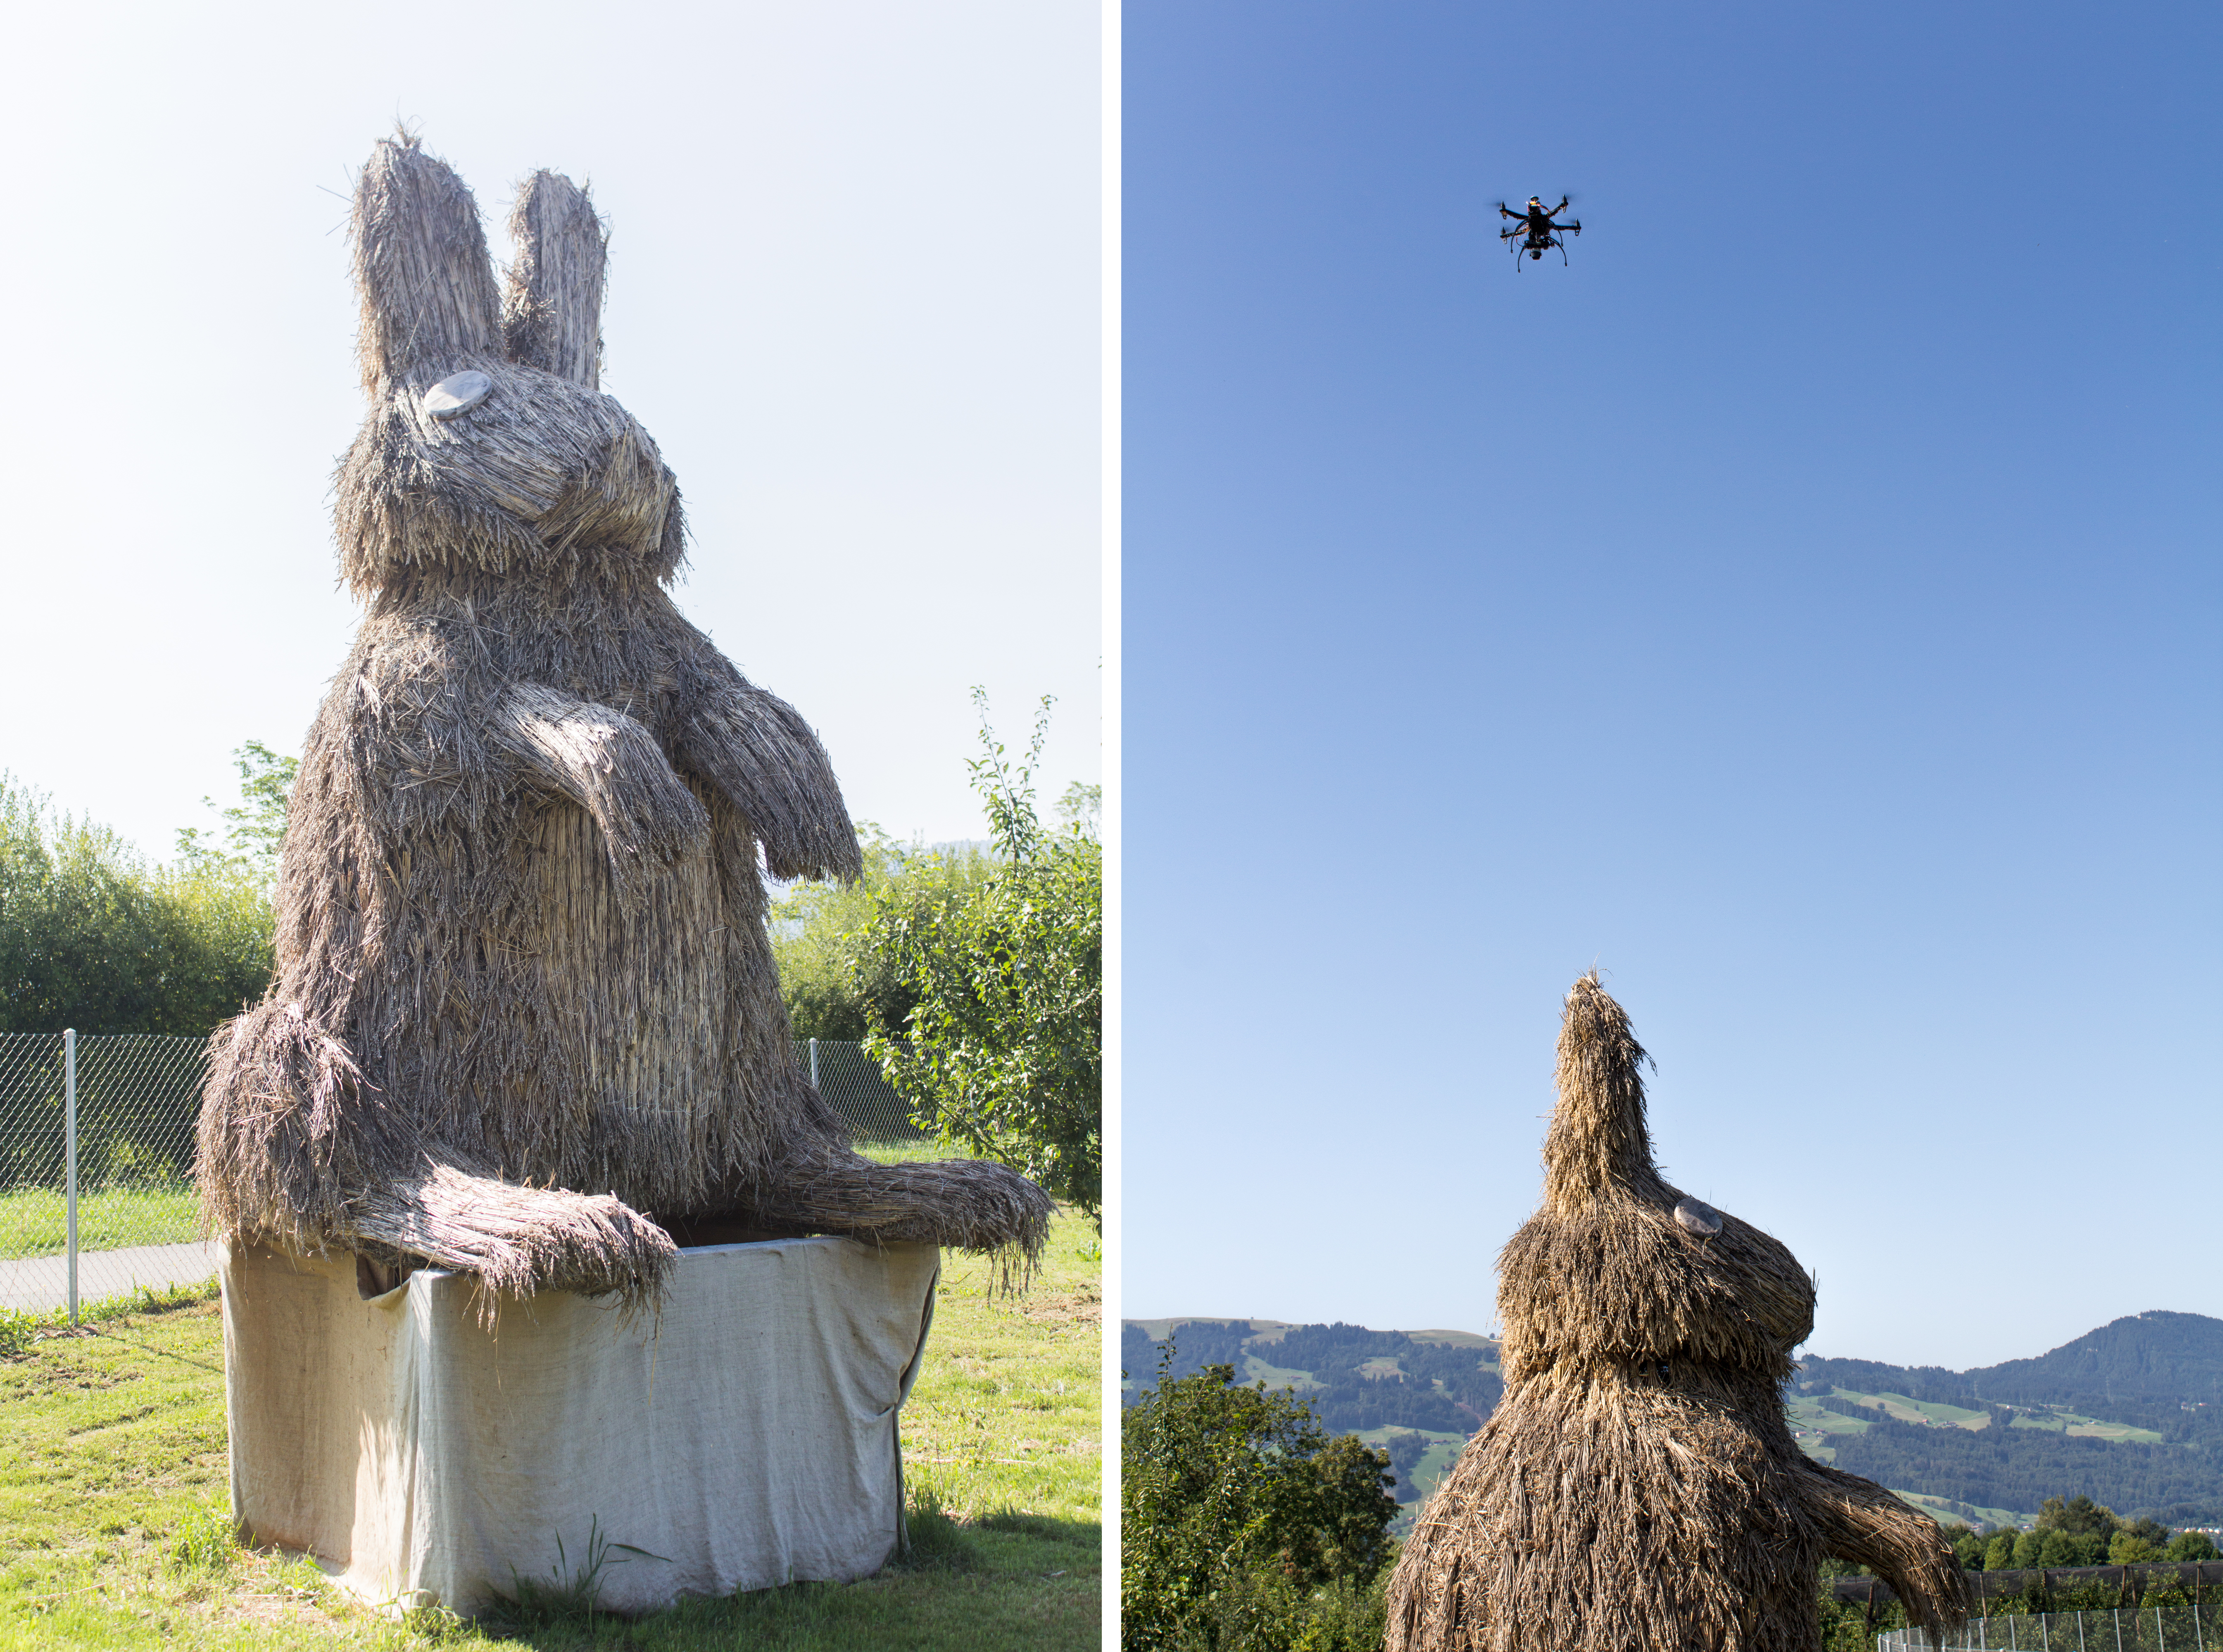
\includegraphics[width=\textwidth]{images/rabbit4.jpg}
	\caption{Der Strohhase}
	\label{img:rabbit4}
\end{figure}

%----------------------------------------------------------------------------------------

\section{Testsystem und -parameter}

Alle 3D-Rekonstruktionen wurden auf einem Intel Core i7 System mit 32 GiB RAM
durchgeführt.   % TODO More cpu details

Die Rekonstruktion wurde in jeder Software mit den Standardeinstellungen
durchgeführt.

%----------------------------------------------------------------------------------------

\section{Resultate}

\subsection{Rekonstruktionsdauer}

Folgende Tabelle vergleicht die Rekonstruktionsdauer für die Sparse Cloud, die
Dense Clound und – wo von der Software unterstützt – das Mesh.

\begin{figure}[H]
	\begin{tabular}[H]{lccc}
		\toprule
		\textbf{Software} & \textbf{Sparse Cloud} & \textbf{Dense Cloud} & \textbf{Mesh} \\
		\midrule
		VisualSFM & 1h 13min & 1h 49min & – \\
		Pix4Dmapper Pro & 1h 40min & 3h 46min & 13min \\
		\bottomrule
	\end{tabular}
\end{figure}

\subsection{Komplexität der Resultate}

\begin{figure}[H]
	\begin{tabular}[H]{lcc}
		\toprule
		\textbf{Software} & \textbf{Punkte in Punktwolke} & \textbf{Vertizes in Mesh} \\
		\midrule
		VisualSFM & TODO & – \\
		Pix4Dmapper Pro & TODO & TODO \\
		\bottomrule
	\end{tabular}
\end{figure}

%----------------------------------------------------------------------------------------
